\documentclass[11pt]{article}
\usepackage{graphicx}
\usepackage{listings}
\usepackage{multirow}
\usepackage{color}
\usepackage[english]{babel}
\usepackage{placeins}
\usepackage{url}
\usepackage{mathtools}
\usepackage{enumerate}
%\usepackage{mylingmacros}

\begin{document}

\newcommand\add[1]{{\textcolor{blue}{ADD: #1}}}
\newcommand\modi[1]{{\textcolor{green}{MODIFIED: #1}}}
\newcommand\remove[1]{{\textcolor{red}{REMOVE: #1}}}
\newcommand\expand[1]{{\textcolor{blue}{EXPAND: #1}}}
\newcommand\review[1]{{\textcolor{green}{REVIEW: #1}}}

\title{Data expansion for semantic classification}

\author{Anna Liednikova\\
Supervisor: Claire Gardent}




\maketitle

\tableofcontents

\clearpage

\section{Introduction}
\label{sec:}
 
This project was set within the framework of a collaboration with the
ALIAE startup whose aim is to develop a chatbot to collect
information from clinical patients. The main idea is to replace
strictly defined surveys by a more natural conversation in order to
let users express themselves freely so that more information could be
collected.

The chatbot consists of two main modules:
\begin{itemize}
\item NLU (Natural Language Understanding): interpreting the user input
\item Dialog Managment: deciding how to respond to the user input and
  generating the system response
\end{itemize}


\begin{figure}[htbp]
\begin{center}
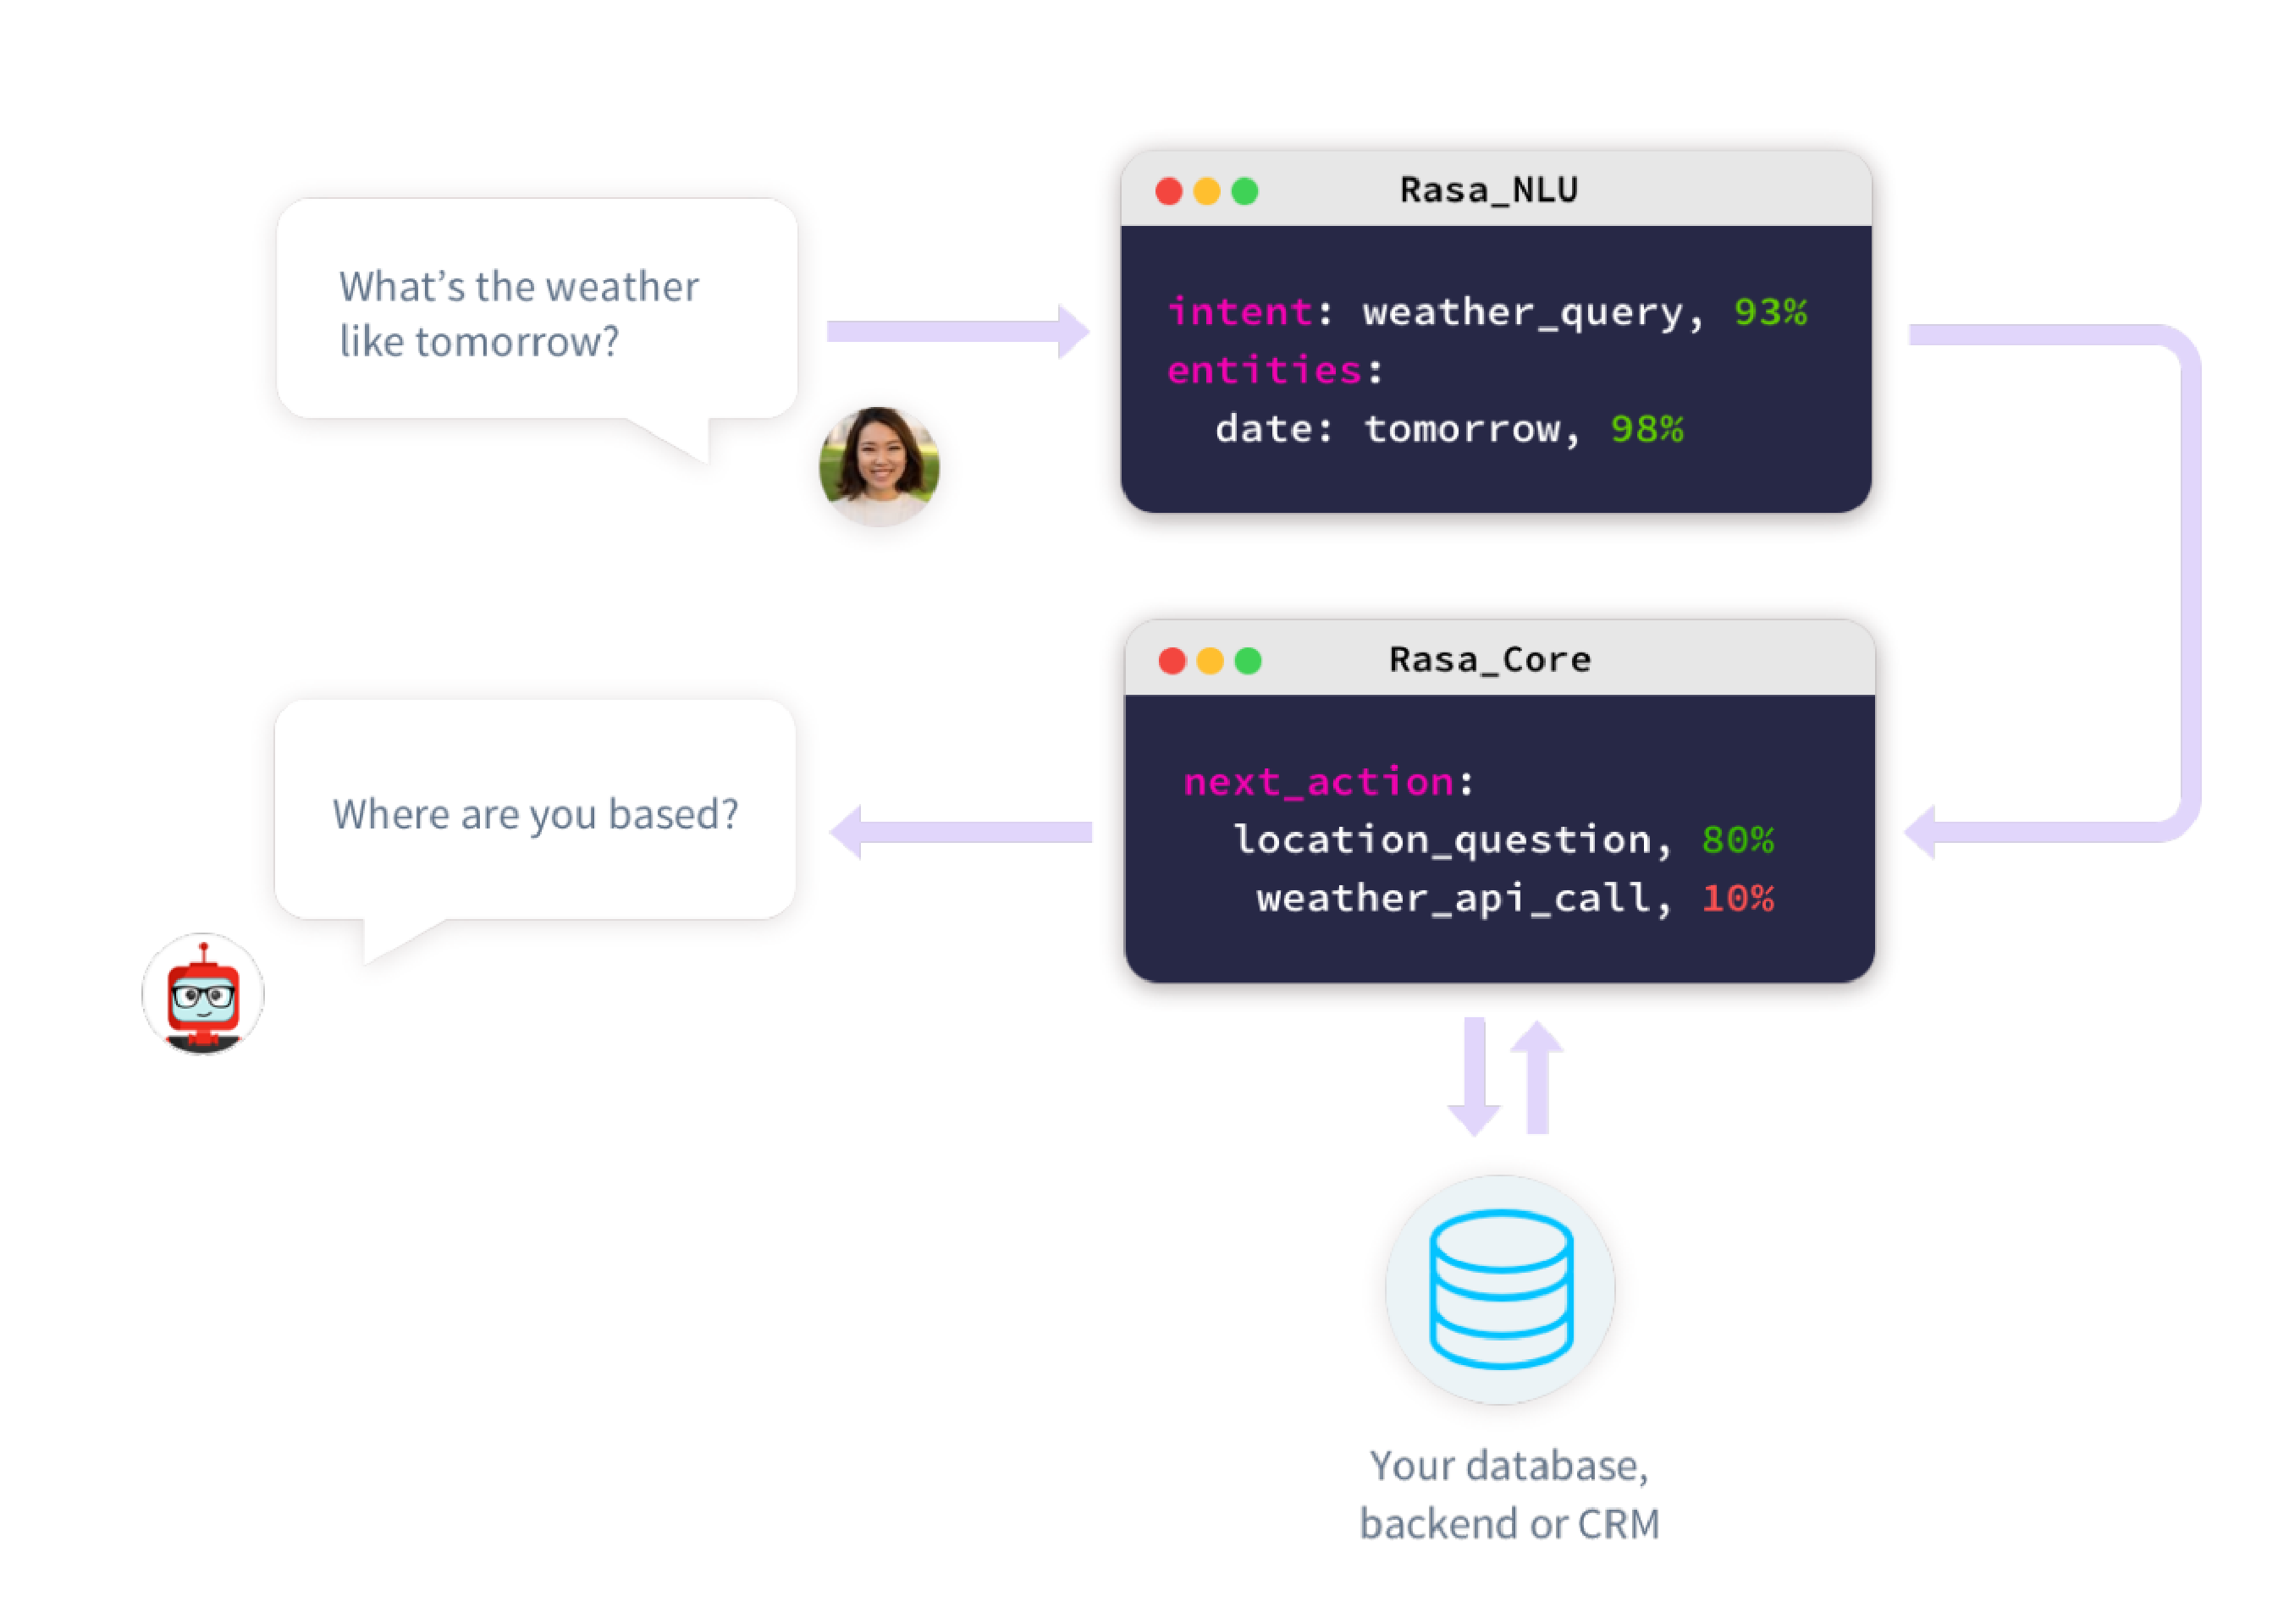
\includegraphics[width=.9\textwidth]{img/rasa.pdf}
\end{center}
\caption{RASA Architecture for Human-Machine Dialog }
\label{fig:rasa}
\end{figure}
In this project, we focus on natural language understanding and
consider a simplified notion of understanding where each user input is
mapped to an ``intent''. Given a pre-defined and finite set of intents
(Does the user speaks about pain, physical activity etc. ), the aim
of the NLU module is to assign each user input an intent\footnote{We
  make the simplifying (and incorrect) assuption that the user input
  contains a single intent.}. The detected intent is then used, in
conjunction with additional information extracted from the previous
dialog interactions, to determine how to
respond (cf. Figure~\ref{fig:rasa}\footnote{The figure
  actually shows a more complex notion of understanding where the user
  utterance is mapped not only to an intent but also to a set of
  entities. In this work, we focus on how to improve intent detection
  and leave entity detection for future research.}).

\section{Goals and Motivations}
\label{sec:goals}


The NLU module is a classifier which given a user input, predicts the
corresponding intent. Our goal is to improve this classifier starting
from a small training set (roughly 100 utterance/intent pair for each
intent) and automatically expanding this labelled data. To this
end, we developed a semi-supervised data expansion technique which
permits expanding the initial data with utterances extracted from a
medical forum. We show that the expanded data permits improving the
classifier by 0.05 accuracty points.

This report is structured as follows. Section~\ref{sec:relatedwork}
briefly reviews the state of the art and situates our proposal with
respect to related work.  Section~\ref{sec:methodology} presents the
methodology used for data expansion. Section~\ref{sec:datasets} describes
the datasets used. Section~\ref{sec:xps} reports on the experimental
setting and on the results. Section~\ref{sec:conclusion} concludes
with pointers for further research.

\section{Related Work}
\label{sec:relatedwork}

To use supervised text classification methods, it is important to have a dataset of a reasonable size in order to make their training efficient. When only a small set of labelled documents is available, the semi-supervised learning becomes a way-out and helps to resolve tasks by comparing the distributions between labelled and unlabelled items.

\cite{N18-2058} presented an approach for automatically generating additional training data for event extraction systems. First, they trained a baseline classifier on available gold data. Then, they split external data into clusters of paraphrases using the NewsSpike method introduced by \cite{zhang2015}. They then label the clusters using the baseline model trained on the initial dataset of labelled data. Combining the new labelled data and the original one, they then retrained the event extractor and achieved significant improvement of F1 score.

There are many models that encode sentences into fixed-size representations. LDA and Word2Vec models have been extensively used and have shown their effectiveness on the continuation of a long time and a wide range of tasks\cite{Iacobacci2016EmbeddingsFW} \cite{Jelodar2017}. Due to their popularity, there are pre-trained models on Tweets and Google News data. Though, the research of \cite{Li2018ComparisonOW} demonstrates that GloVe embeddings trained on the specific data produce better results in narrow field problems than the pre-trained ones that are better for more wide tasks. \cite{P18-1198} also showed the efficiency of BiLSTM-max model for capturing word context in encoding sentences.

SVM is considered to be a hands-on approach in textual classification \cite{SVM} that tends to perform better than other traditional models regardless of the word embedding type \cite{Li2018ComparisonOW}. These classifiers are fast, reliable, work well in both linear and non-linear separation and can effectively deal with sparse data, and have a great ability to generalize knowledge in multidimensional spaces \cite{joachims98a}. Last two advantages especially important due to the common use of high dimension in sentence representation task and its sparse nature in case of LDA.

\section{Methodology}
\label{sec:methodology}

Our methodology for data expansion falls into two main steps. First, we compare different methods for representing utterances using both clustering and classification (Section~\ref{subsec:sentencerepresentations}). Second, based on the best sentence representations, we devise a semi-supervised approach which relies on clustering and classification to gradually increment the size of the labelled data and iteratively train new classifiers on the extended data (Section~\ref{subsec:dataexpansion}). 

%% We follow \cite{N18-2058} methodology. Instead of using \cite{zhang2015}'s methods for identifying clusters of related sentences however, we explore different ways of representing sentences using deep learning approaches. We then apply clustering to the resulting sentence representations. Finally, we investigate the impact of the extended labeled data on classification. 

%% irst
% group together paraphrases of event mentions.

%% then use the simple examples in each cluster to as-
% sign a label to the entire cluster

%% com-
% bine the new examples with the original training
% set and retrain


\subsection{Building and Evaluating Sentence Representations}
\label{subsec:sentencerepresentations}

We investigate different ways of creating continuous representations for sentences and use clustering to determine which representation best support the identification of intents. 

\subsubsection{Creating Continuous Representations of Sentences.}

We explore two ways of building sentence representations: Word2vec and LDA. %% he good point of using these models is that they can be used for both word and sentence representation since one word can be treated as a small sentence. That can help us also to create sentence representations in two steps using machine and deep learning techniques. First, we map words to continuous representations. Second, we combine these word representations into sentence representations using BiLSTM encoder. \add{bibref}.

%We construct sentence representations out of the word representations described in the previous section using two types of neural networks:  PositionwiseFeedForward \cite{vaswani2017attention} and BiLSTM \add{bibref}.

\paragraph{LDA.}

One of the most common methods for constructing thematic models is the Latent Dirichlet Allocation (LDA) $\cite{lda_def}$ that models a document as a distribution of topics and a topic as a distribution of words. Here a document is a sentence. Hence a sentence is represented as a distribution of topics. 

Let's consider a toy LDA model produces following topics:

\begin{lstlisting}
[(0,
  '0.089*"_num_" + 0.025*"day" + 0.022*"pain" + 0.020*"take" + 
   0.018*"year" + 0.017*"feel" + 0.015*"smoke" + 0.014*"sleep"'),
 (1,
  '0.024*"good" + 0.022*"get" + 0.021*"feel" + 0.021*"blood" + 
   0.021*"want" + 0.020*"pressure" + 0.014*"understand" '),
 (2,
  '0.067*"go" + 0.048*"sleep" + 0.023*"_num_" + 0.021*"bed" + 
   0.018*"fall" + 0.018*"hour" + 0.017*"wake" + 0.016*"asleep" '),
 (3,
  '0.040*"drink" + 0.030*"life" + 0.025*"much" + 0.020*"eat" + 
   0.017*"end" + 0.016*"go" + 0.013*"time" + 0.012*"body" ')]
\end{lstlisting}


And here is an example representation for a  sentence/ 

\begin{lstlisting}
'I can go for months and at least a year or so without drinking',
[0.61565   , 0.03821149, 0.32365379, 0.02248472]
\end{lstlisting}

If we want represent just one word we can just treat it like a small sentence and have the same output.
\begin{lstlisting}
'sleep',
[(0, 0.21281178), (1, 0.13255174), (2, 0.5765724), (3, 0.07806411)]
\end{lstlisting}

The LDA algorithm is based on the Dirichlet prior distribution and
assumes a bag-of-words model - a model for analyzing texts
that takes into account only the frequency of words, but not their
order. This model is well suited for thematic modeling, since it
permits detecting implicit relationships between words. The LDA
method performs soft clustering and assumes that each word in the
sentence is generated by some latent topic, which is determined by a
probability distribution on the set of all words of the text.


\paragraph{Word2Vec.} Word2Vec representations are low dimensional vectors also called embeddings which are built based on textual
cooccurences and learned using shallow, two-layer neural networks
\cite{Mikolov2013EfficientEO}. Given a large corpus of text as input,
Word2Vec produces a vector space where words that share common
contexts in the input corpus will be mapped to vectors that are close
to one another in the vector space.


To build sentence representations, we simply average the Word2Vec
vectors of the content words present in that sentence.

\paragraph{Bi-LSTM.} The general idea of BiLSTM layer is repeating the first recurrent layer in the network so that they are next to each other and then providing the straigh input sequence as input to the first level and an inverse copy of it for the second.

In more formal way, for the sequence of words $T \{w_{t}\}_{t = 1, ..., T}$ bidirectional LSTM computes a set of T vectors $\{h_{t}\}_{t}$. For $t ∈ [1 ,. ,,, T]$, $h_{t}$ is the combination of forward and backward LSTM, that read sentences in two opposite directions. 

We experiment with two ways of combining a changing number $(h_{1}, ..., h_{T})$ to form a vector of a fixed size, either by choosing the last hidden state $h_{T}$ (BiLSTM-last), or either by selecting the maximum value over each dimension of the hidden units (max pooling) (Collobert and Weston, 2008) or by considering the average of the representations (mean pooling). The choice of these models is motivated by their demonstrated effectiveness in embedding models \cite{P18-1198}.


\subsubsection{Evaluating Sentence Representations Using Clustering}

Using the sentence representations described in the previous section,
we apply clustering to group together sentences that are similar.  We
set the number of clusters to the number of intents (20) and we use
(i) purity and Silhouette coefficients to evaluate the clusters
 and (ii) homogeneity and completeness to better assess how the
resulting clusters correlate with initial intents. Also, for each
model, we plot a confusion matrix with a background gradient to
visualize how well clusters separate different intents. Based on these
metrics and vizualisation, we determine which method produces
representations that best support intent detection.

We compare three clustering algorithms:

\begin{itemize}
\item K-Means (KM)
\item Agglomerative Clustering (AG)
\item Gaussian Mixture (GM)
\end{itemize}


\paragraph{K-Means.} The basic idea is to define K centroides one for each cluster. It is best to place them as far apart as possible. The next step will be to accept each point belonging to this data set and associate it with the precision of the centroid. If no point is under consideration, the first stage is completed. At the moment, we need to re-calculate K's new centroids, as the cluster barycenter that stems from the previous step. After these new centroids appear on us, a new binding must be made between the same points of the data set and the nearest new center of gravity. A loop is created. As a result of this cycle, we can see that k centroids change their location step by step until any changes are made. In other words, centroids are no longer moving.

The algorithm is aimed at minimizing the target function, in this case, the quadratic error function. Target function:
\begin{equation}
J = \sum_{j=1}^{k} \sum_{i=1}^{n} (\Vert x_{i}^{(j)} - c_{j} \Vert)^{2}
\end{equation}

where $(\Vert x_{i}^{(j)} - c_{j} \Vert)^{2}$ is the chosen distance between the data point $x_{i}^{(j)}$ and center $c_{j}$, it is an indicator of the distance n of the data points from their respective cluster centers.

Centroid is defined as follows:

\begin{equation}
c_{j} = \dfrac{1}{N} \sum_{i=1}^{N} x_{i}^{(j)}
\end{equation}

where $x_{i}^{(j)}$ is the point belonging to the cluster $J$, $N$ - total number of points in the cluster.

\paragraph{Agglomerative Clustering} is a kind of hierarchical clustering with 'bottom-up' approach when new clusters are created by combining smaller clusters and, thus, a tree is created from leaves to trunk \cite{ward63:_hierar_group_optim_objec_funct}. The main feature of the agglomerative hierarchical clustering method is that if we want to get a different number of clusters, we will not need to restart the algorithm, because the whole tree is calculated, and then we say that we want to cut it in some place.


Different linkage criterions can be used to calculate distance between sets of observation. Ward’s method minimizes the variance of the clusters being merged. This method is used for tasks with closely spaced clusters. The euclidian distance between clusters is taken as the increment of the sum of squares of the distances of objects to the center of the cluster, obtained as a result of their combination: 

\begin{equation}
\Delta = \sum_{i} {(x_{i} - {\bar {x}})^{2}} - \sum_{x_{i} \in A} (x_{i} - {\bar {a}})^{2} - \sum_{x_{i} \in B} (x_{i} - {\bar {b}})^{2}
\end{equation}

At each step of the algorithm, these two clusters are combined, which lead to a minimal increase in variance.



\paragraph{Gaussian Mixture.}

In statistics, a mixed model is a probabilistic model for representing the presence of subpopulations in the general population in accordance with the mixture of distributions, without requiring that a separate observation belong to a specific subgroup.

A Gaussian mixture model \cite{reynolds2015gaussian} represents a weighted sum of M Gaussian densities elements for D-dimensional continuous-valued data vectors:

\begin{equation}
p(x|\lambda) = \sum_{i=1}^{M} w_{i} g(x|\mu_{i}, \sum_{i})
\end{equation}

where each Gaussian densities element defined as 

\begin{equation}
g(x|\mu_{i}, \sum_{i})=\frac{1}{(2\pi)^{\frac{D}{2}}|\sum_{i}|^{\frac{1}{2}}} e^{-\frac{1}{2}(x-\mu_{i})'\sum_{i}(x-\mu_{i})} 
\end{equation}

with mean vector $\mu_{i}$ and covariance matrix $\sum_{i}$. The mixture weights satisfy the constraint that $\sum_{i=1}^{M} w_{i} = 1$.

GMM parameters are estimated from training data using the iterative Expectation-Maximization (EM) algorithm or Maximum A Posteriori (MAP) estimation from a well-trained prior model.


\subsection{Semi-Supervised approach to Data Expansion and Classification}
\label{subsec:dataexpansion}

Based on experimental results (cf. Section~\ref{sec:xps}), we choose
the best model for representing sentences. We then use these
representations to iteratively expand the training data and train the
corresponding classifiers based on the following procedure:


\begin{itemize}
\item \textbf{Step 1: Classification.} Apply the classifier trained on the currently available labelled data to a set of unlabelled sentences;
\item \textbf{Step 2: Clustering.} Clusterize these unlabelled sentences into 200 clusters
\item \textbf{Step 3: Filtering.} Use the probability and the label assigned by the classifier to each unlabelled sentence to :
  \begin{itemize}
\item Eliminate sentences whose probability is below a given threshold
\item Eliminate clusters with less than a set number of members
  \end{itemize}
\item \textbf{Step 4: Data expansion.} For each intent, add the $n$ best labelled items to the training data.
  \item \textbf{Step 5: Classifier Training.} Train a new classifier using both the previous and the newly selected, labelled data. 
\end{itemize}

\subsubsection{Classification.} For classification, we use SVC (Support Vector Classifier). The main idea of ​​the method is transfering the initial vectors into a space of higher dimension and searching for a separating hyperplane with the maximum gap in this space. Two parallel hyperplanes are built on both sides of the hyperplane separating the classes. The separating hyperplane will be the one that maximizes the distance to two parallel hyperplanes. The algorithm works under the assumption that the greater the difference or the distance between these parallel hyperplanes, the less will be the average classifier error.  Due to the small size for dataset it's essential to create balanced training and test datasets.

The initial labelled dataset was provided by ALIAE (gold data). We split our gold dataset into train and test sets and systematically use the test set for evaluation and comparison of the classifiers learned on the different datasets produced during data expansion.

At each iteration during data expansion, we use the classifier trained
on the data created at the previous iteration to label unlabelled
sentences extracted from some external source. 

\subsubsection{Clustering.} To expand the training data, we retrieve utterances from a medical forum. The unlabelled data is then built based on these utterances after some filtering is applied to eliminate sentences that are either out of topic or too complex (cf. Section~\ref{sec:}). Next we build representations for these unlabelled sentences using the techniques described in Section~\ref{sec:} and we apply clustering to create 200 clusters. 

\subsubsection{Filtering.} The SVC classifier assigns each unlabelled sentence a category (an intent) and a probability. We eliminate from the clusters all those sentences whose probability is below a given threshold. We then eliminate all clusters whose size is less than a set minimum. 

For our subset we find the best clusterization by elbow method \cite{elbow_rule}. Later, having both labels for intent and cluster, we leave just that clusters that populated by items with maximum probability that allows us to cover all intent with new examples.

For each cluster we calculate number of intent representators and their overall distribution. We then keep only those clusters where some intent is represented more than in average. Elements of clusters that are left will be labelled by the majority.


\subsubsection{Data Expansion.} Finally, we select N labelled items for each category/intent and extend the training data with them to update sentence representation and classification models.

We repeat this cycle until we won't be able to extend train dataset by additional samples or classifier score will stop to grow.

\section{Datasets}
\label{sec:datasets}

For our task we have two datasets: a small, manually labelled dataset
where each utterance is associated with a target intent; and a large,
unlabelled dataset extracted from the web. Our goal is to
automatically label this web data in order to expand the training set
and to improve the NLU module of the ALIAE chatbot.


\subsection{Labelled Data}
\label{subsec:labelleddata}
The initial dataset was created manually by the Aliae startup and  covers 20 main possible users intents. Each sentence represents one intent e.g., 
%\enumsentence{
\begin{description}
\item[Text:] After sleep, for 2-3 hours, I am better and then start feeling tired again
\item[Intent:] sleep
\end{description}
%}

The distribution of labels is shown in Figure~\ref{figure:name}. There
are in average, 3.4 words per sentence (min: 0, max: 12, std:
2.16367).  The total number of sentences is 3305 and the vocabulary
consists of 1882 content words (after removing stopwords).

 \begin{figure}[h]
 	\centering
 	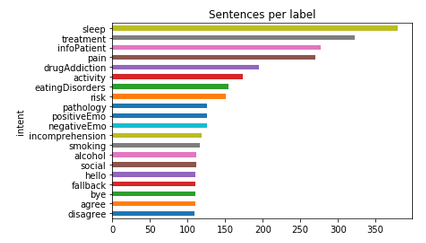
\includegraphics[scale=0.4]{report1.png}
	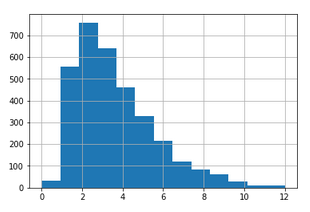
\includegraphics[scale=0.45]{report4.png}	
	\caption{Left: Label distribution in dataset, Right: Distribution of sentence length}
 \label{figure:name}
 \end{figure}
\FloatBarrier


\subsection{Unlabelled Forum data}
\label{subsec:forumdata}

To improve the initial classifier, we needed to extend the training
dataset by much more data and more naturally constracted one. Looking
for open medical dataset that can be used for this purpose, we found
\cite{zhang2015} and \cite{sondhi-EtAl:2010:POSTERS} works that used
the HealthBoards forum data for similar tasks. 
HealthBoards\footnote{\url{healthboards.com}} is a medical forum web portal that
allows patients to discuss their ailments.


We scraped 272553 unique posts labelled with 238 forum
categories. Figure~\ref{forum_data_stat} shows the dataset
statistics. In average, sentences contain $11\pm7$ words after
preprocessing.


 \begin{figure}[h]
 	\centering
 	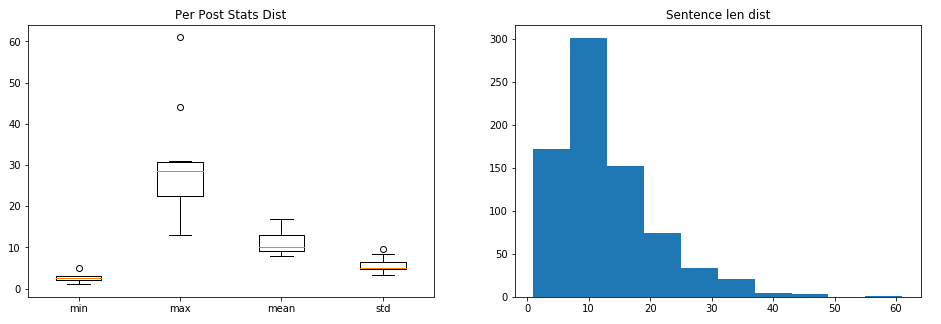
\includegraphics[scale=0.4]{report3.png}
	\caption{Text stat}\label{forum_data_stat}
 \end{figure}
\FloatBarrier

This dataset has its own categorization so that some posts are more specialized and some are out of the scope of our intent labels. We should start with the data that is most similar to the initial one, so that's why we choose post categories hich are similar to our intents. This will help us to gradually expand the training data. So we will keep posts of categories provided in table \ref{cat_freq}.

\begin{table}[htb]
\centering
\begin{tabular}{ |r|c| }
\hline
Category of board &  \# of posts \\ \hline
digestive-disorders & 5064 \\ \hline
addiction-recovery & 3644 \\ \hline
sleep-disorders & 1748 \\ \hline
smoking-cessation & 937 \\ \hline
eating-disorder-recovery & 762 \\ \hline
chronic-pain & 735 \\ \hline
chronic-fatigue & 662 \\ \hline
stress & 415 \\ \hline
family-friends-addicts-alcoholics & 312 \\ \hline
pain-management & 25 \\ \hline
\end{tabular}
\caption{Selected Forum categories}\label{cat_freq}
\end{table}
\FloatBarrier

Finally, the corpus consists of 380014 sentences. 

Also, for big number of iterations, the data should be divided in
subsets by increasing sentence length because of the difference in
mean values for both datasets. So after tokenizing tje posts into
sentences we calculate their length. For each iteration, we only keep
those sentences which have mean+std words after pre-processing
(cf. Section~\ref{subsec:preprocessing}).


\section{Experiment}
\label{sec:xps}

We now describe how the steps described in Section~\ref{sec:methodology} were applied to the forum data.

%% Experiment consists of the main stages:

%% \begin{itemize}
%% \item preprocess text of labelled and unlabelled data
%% \item use clustering to choose between different ways of representing sentences
%% \item training a classifier on the labelled data
%% \item iterative semi-supervised learning:
%%   \begin{itemize}
%%   \item data expansion (cf Section \ref{subsec:dataexpansion}) ; 
%%   \item update sentence representations (using new data and old parameters)
%%   \item retrain on classifier on gold + new labelled data
%%   \item evaluate new classifier on gold test data
%% \end{itemize}
%% \end{itemize}

\subsection{Preprocessing }
\label{subsec:preprocessing}

To build continuous representations of sentences, we only take into
account the lemmatized form of the content words they contained. Hence
a pre-processsing step is applied to segment the forum data into
sentences, to tokenize and lemmatize the resulting sentences and to
remove stop words.

For lemmatization we used SpaCy as it provides lemmas for every token. Next examples shows the transformation:

\begin{quote}
Before: 	I can go for month\textbf{s} and at \textbf{least} a year or so without drink\textbf{ing} \\
After: 		I can go for month and at little a year or so without drink
\end{quote}

We compared two libraries, NLTK and SpaCy for tokenization, they give different results that can influence not only simple statistics but also meaning. Some example of different tokenizations can be seen in table \ref{token_dif}. Although tokenizing  words such as 'flulike' or '35mg' or 'longterm' sometimes gives more robust and concrete meaning, in our case it seems better to stay with SpaCy way of tokenization in order to have a smaller and simpler vocabulary.

\begin{center}
\begin{table}
\begin{tabular}{ |p{7cm}|p{7cm}| }
\hline
NLTK & SpaCy \\ \hline
['i', 'wouldnt', 'go', 'to', 'sleep', 'until', 'like', '5', '6', 'or', '8am'] & 
['i', 'would', 'nt', 'go', 'to', 'sleep', 'until', 'like', '5', '6', 'or', '8', 'am'] \\ \hline
['that', 'is', 'totally', 'wrongheaded'] & ['that', 'is', 'totally', 'wrong', 'headed'] \\ \hline
['i', 'am', 'in', 'the', 'process', 'of', 'tapering', 'from', 'suboxone', 'longterm', 'use'] & 
['i', 'am', 'in', 'the', 'process', 'of', 'tapering', 'from', 'suboxone', 'long', 'term', 'use'] \\ \hline
['i', 'had', 'an', 'onandoff', 'opiateopioid', 'habit', 'from', 'about', '2010'] & 
['i', 'had', 'an', 'on', 'and', 'off', 'opiate', 'opioid', 'habit', 'from', 'about', '2010'] \\ 
\hline
['i', 'have', 'flulike', 'pathologysymptom'] & ['i', 'have', 'flu', 'like', 'pathologysymptom'] \\ \hline
['i', 'have', 'exerciseinduced', 'insomnia'] & ['i', 'have', 'exercise', 'induced', 'insomnia'] \\ \hline
['i', 'm', 'supposed', 'to', 'take', '6', '35mg', 'tablets', 'a', 'day', 'but', 'i', 'have', 'taken', '20', 'today'] & 
['i', 'm', 'supposed', 'to', 'take', '6', '35', 'mg', 'tablets', 'a', 'day', 'but', 'i', 'have', 'taken', '20', 'today'] \\ 
\hline
\end{tabular}	
\caption{Tokenization comparison}\label{token_dif}
\end{table}
\end{center}
\FloatBarrier

For stopwords removal, there were three options: NLTK, SpaCy and the
longest one. The last option was rejected due to containing words like
'want', 'stop', 'successfully' etc. that can be useful for detecting
basic intents such as social (e.g., greetings) and positive or
negative emotions. In the end, we decided to use NLTK because of
containing shorts like 'm' from 'am', 've' from 'have'.

The final dictionary contained 1882 words. Also all numbers were
changed to {\sc{num}}. Figure~\ref{words_freq} shows the distribution of word frequency. 

 \begin{figure}[h]
 	\centering
 	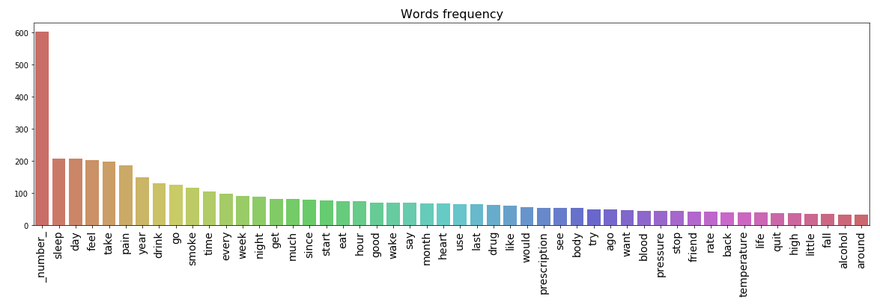
\includegraphics[scale=0.4]{report2.png}
	\caption{Words frequency}
 \label{words_freq}
 \end{figure}
\FloatBarrier

%% Next problem we faced is empty sentences. But there is not a lot of occurances, so their dropping don't change the dataset much.

%% \begin{tabular}{ |r|l| }
%% \hline
%% intent & items \\ \hline
%% fallback          & 12 \\ \hline
%% disagree          & 11 \\ \hline
%% hello             &  4 \\ \hline
%% agree             &  3 \\ \hline
%% incomprehension   &  2 \\ \hline
%% positiveEmo       &  1 \\ \hline
%% \end{tabular}

%% These sentences are: 'what?', 'same that again', 'I am up', 'same', 'can you',
%%        'do that', 'do this', 'Will do', 'no', 'no i will not',
%%        "No i don't", 'no', 'no i will not', "No i don't", "What's up?",
%%        "What's up?", 'he', 'a', 'd', 'i', 'm', 'o', 's', 't', 'y',
%%        'I will', 'Will do', 'No', 'no', 'No it is not', "No I don't",
%%        'No', "I'm here"


\subsection{Clustering for sentence representation evaluation}
\label{subsec:clustering2}

We use clustering to assess the degree to which sentence representations support the correct classification i.e., the assignment of the correct intent. Also, clustering provides us with information about which classes will be easier to identify and which can mix with others. Using evalution metrics for clustering helps us to compare different ways of representing sentences and to chose the best one.

For each type of sentence representations described in
Section~\ref{sec:}, we split the forum data  into 20 clusters
which corresponds to the number of intents. To select the best model,
we further experiment with different hyper-parameters (number of topics for
LDA and embedding size for Word2Vec).
%The preferred number of features for Word2Vec model is 200. It's the start point for our model.

\subsubsection{Evaluation metrics}

For every model, we compute the following metrics and their average:
purity score, Silhouette Coefficient, homogeneity and completeness
scores.
%Later for each parameter average among clustering models calculated for each score in order to get both table and plot.

Also for each model, we create the confusion matrix between cluster labels and target intents.

\paragraph{Purity} is calculated by assigning each cluster to the class that is most often found in the cluster, and then the accuracy of this assignment is measured by counting the number of correctly assigned documents and dividing by N.

\begin{equation}
\centering
purity(\Omega,C) =\frac{1}{N} \sum_{k} \max_{j}|\omega_{k}\cap c_{j}|
\end{equation}
where $\Omega=\{\omega_{1}, \omega_{2}, ... ,\omega_{K}\}$ is the set of clusters and $C = \{c_{1}, c_{2}, ... , c_{J}\}$ is the set of classes. 

\paragraph{Silhouette Coefficient} shows how much the average distance to objects of its cluster differs from the average distance to objects of other clusters. This value is in the range $\lfloor 0, 1\rfloor$. Values close to -1 correspond to poor (scattered) clustering, values close to zero indicate that the clusters intersect and overlap each other, values close to 1 correspond to "dense" clearly selected clusters. Thus, the larger the silhouette, the more clearly highlighted the clusters, and they are compact, tightly grouped clouds of points.

\paragraph{Homogeneity and completeness.} Homogeneity will be maximal if the cluster consists only of objects of one class. Completeness will be maximum if all objects from the class belong to only one specific cluster.
Formally, these measures are also determined using the functions of entropy and conditional entropy, considering the partitioning of the sample as discrete distributions:

\begin{equation}
h = 1 - \frac{H(C|K)}{H(C)}, c = 1 - \frac{H(K|C)}{H(K)}
\end{equation}

here is $K$ the result of clustering, is $C$ the true partitioning of the sample into classes. Thus, $h$ measures how much each cluster consists of objects of one class, and $c$ measues how much objects of one class belong to one cluster.

\subsubsection{Word2Vec model}

For Word2Vec representations, we compare results for 
embedding sizes ranging from 10 to 600.

\begin{center}
\begin{tabular}{ |c|c|c|c|c|c| }
\hline
Embedding Dim.  & purity  & silhouette  & homogeneity  & completeness\\ \hline 
10  & 0.179526  & 0.0767427  & 0.106067  & 0.12561\\ \hline 
20  & 0.185678  & 0.0873321  & 0.107696  & 0.132483\\ \hline 
30  & \textbf{0.189007}  & 0.0695026  & 0.110232  & 0.13267\\ \hline 
50  & 0.180535  & 0.0441912  & 0.110117  & 0.131568\\ \hline 
100  & 0.186788  & 0.0594827  & \textbf{0.11196}  & 0.139803\\ \hline 
150  & 0.184569  & 0.0427566  & 0.107914  & 0.141453\\ \hline 
200  & 0.179425  & 0.0504081  & 0.103741  & 0.13929\\ \hline 
300  & 0.174382  & 0.047393  & 0.102877  & 0.147216\\ \hline 
400  & 0.175391  & 0.0520504  & 0.103353  & \textbf{0.153824}\\ \hline 
500  & 0.171659  & 0.0443621  & 0.0973479  & 0.153174\\ \hline 
550  & 0.170449  & \textbf{0.11301}  & 0.099802  & 0.133441\\ \hline 
600  & 0.171357  & 0.0593728  & 0.0977992  & 0.151583\\ \hline 
\end{tabular}
\end{center}
\FloatBarrier

\begin{figure}[h]
\centering
 	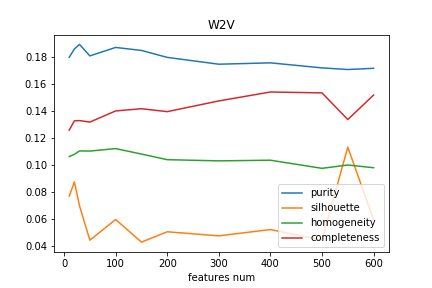
\includegraphics[scale=0.7]{w2v_scores.png}
	\caption{Word2Vec scores}
\label{w2v_scores}
\end{figure}
\FloatBarrier

Scores don't provide clear choice, so let's look at confusion matrixes of models with 30 (Figure \ref{w2v30_cm}) and 100 dimension vector (Figure \ref{w2v100_cm}) that have the highest scores for purity and homogeneity. As we can see from figures models tends to put most of the items into two general clusters: social-like (agree, bye, fallback, hello) and others. KMeans clusterization for W2V with 30 dimensions seems to have more separated groups, so it will be left for further selection.

\begin{figure}[h]
	\centering
	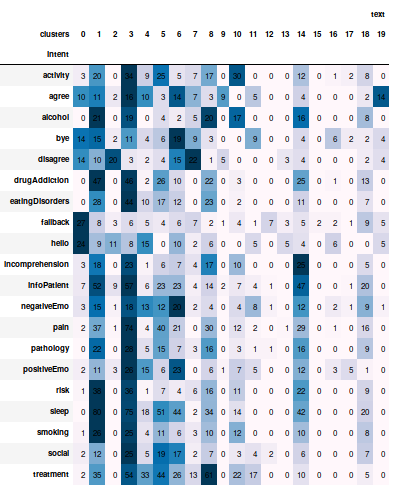
\includegraphics[scale=0.28]{w2v30_ac.png}
	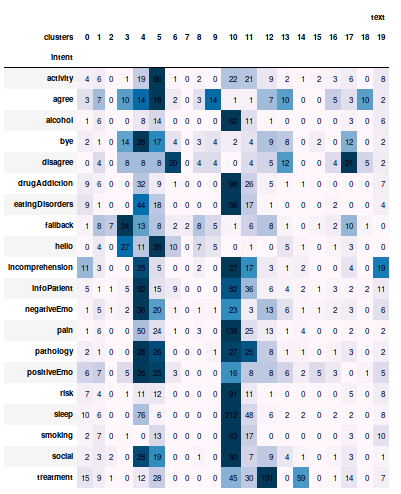
\includegraphics[scale=0.28]{w2v30_gm.png}
	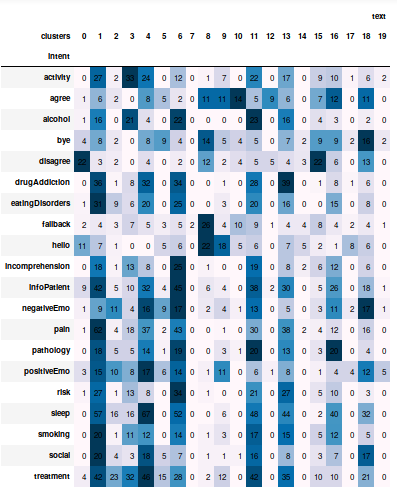
\includegraphics[scale=0.28]{w2v30_km.png}
	\caption{30 dimension W2V confusion matrixes: agglomerative clustering, gaussian mixture, Kmeans}
\label{w2v30_cm}
\end{figure}
\FloatBarrier

\begin{figure}[h]
	\centering
	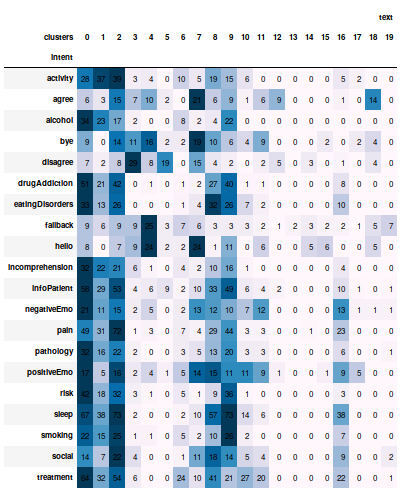
\includegraphics[scale=0.28]{w2v100_ac.png}
	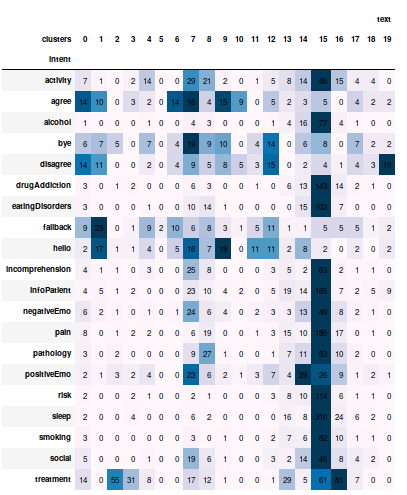
\includegraphics[scale=0.28]{w2v100_gm.png}
	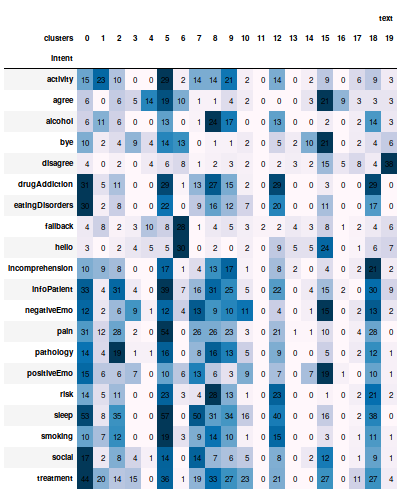
\includegraphics[scale=0.28]{w2v100_km.png}
	\caption{100 dimension W2V confusion matrixes: agglomerative clustering, gaussian mixture, Kmeans}
\label{w2v100_cm}
\end{figure}
\FloatBarrier


\subsubsection{LDA model}
\label{subsec:lda}

For LDA representations, we iterated through different numbers of
topics for LDA model to see which one should be used to represent our
dataset. Table~\ref{LDA_num_topic} shows the results. 

\begin{table}[htb]
\begin{center}
\begin{tabular}{ |c|c|c|c|c| }
\hline
num & purity  & silhouette  & homogeneity  & completeness \\ \hline 
10  & 0.253656  & 0.461589  & 0.157498  & 0.178928  \\ \hline 
20  & 0.259203  & 0.378276  & 0.168191  & 0.182203  \\ \hline 
30  & 0.251538  & 0.331069  & 0.157755  & 0.168448  \\ \hline 
50  & 0.240545  & 0.287032  & 0.147430  & 0.166824  \\ \hline 
100  & 0.266465  & 0.187596  & 0.168647  & 0.189221 \\ \hline 
150  & 0.256077  & 0.167888  & 0.161589  & 0.185054 \\ \hline 
200  & 0.263843  & 0.149212  & 0.175117  & \textbf{0.194913} \\ \hline 
300  & 0.250025  & 0.151526  & 0.165607  & 0.184314 \\ \hline 
400  & \textbf{0.272718}  & 0.192777  & \textbf{0.177547}  & 0.192270 \\ \hline 
500  & 0.259506  & \textbf{0.203725}  & 0.174925  & 0.192831 \\ \hline 
550  & 0.229450  & 0.166200  & 0.149270  & 0.158548 \\ \hline 
600  & 0.254261  & 0.191729  & 0.171744  & 0.186001 \\
\hline 
\end{tabular}
\caption{Comparison of LDA with different number of topics}
\label{LDA_num_topic}
\end{center}
\end{table}
\FloatBarrier

The best model is LDA with 400 topics according to scores and with priority to purity and homogeneity ones as it's more important for us to have one intent in one cluster even if some intents will be present in several ones.

\begin{figure}[h]
	\centering
	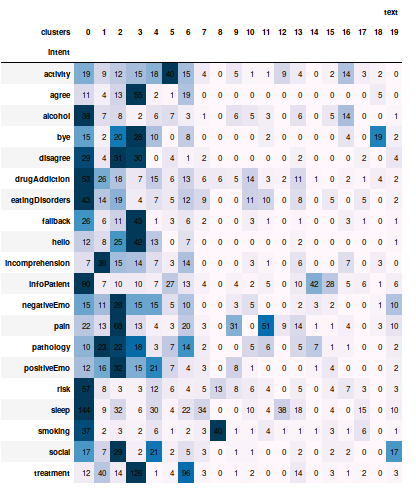
\includegraphics[scale=0.28]{lda_ac_cm.png}
	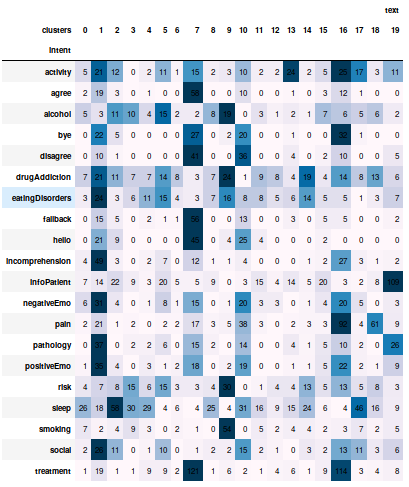
\includegraphics[scale=0.28]{lda_gm_cm.png}
	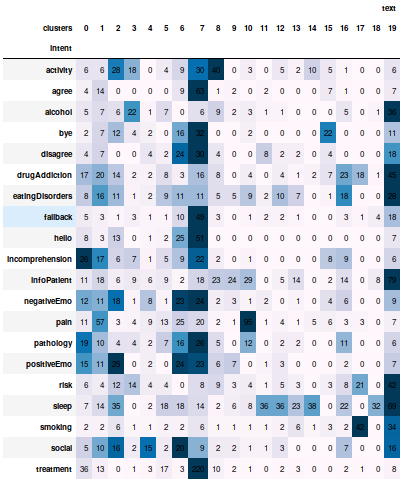
\includegraphics[scale=0.28]{lda_km_cm.png}
	\caption{LDA confusion matrixes: agglomerative clustering, gaussian mixture, Kmeans}
\label{lda_gm_cm}
\end{figure}
\FloatBarrier

The confusion matrix between clusters and intent labels helps us make
hypotheses about possible errors and difficulties and figure out what
connections our model distinguishes well. Thus, although there are
differences between the confusion matrices shown for the three
clustering algorithms, they all show a reccurrent set of errors. In
particular, the following intent are incorrectly clustered together:
fallback and hello; alcohol, drugAddiction and risk; social and
emotions.

\subsubsection{BiLSTM by word}

Following \cite{P18-1198} we trained BiLSTM encoder model experimenting with different hyper-parameters such as  the number of layers, the dimension of the word embedding and the type of pooling.

\begin{table}[htb]
\begin{center}
\begin{tabular}{ |r|c|c|c|c|c| }
\hline
layers & purity  & silhouette  & homogeneity  & completeness \\ \hline 
1  & \textbf{0.286369}  & 0.239979  & \textbf{0.227069}  & \textbf{0.232338}\\ \hline 
2  & 0.262836  & 0.181804  & 0.211068  & 0.219279\\ \hline 
3  & 0.238284  & 0.266460  & 0.195002  & 0.206703\\ \hline 
4  & 0.218623  & \textbf{0.439161}  & 0.164478  & 0.192599\\ \hline 
\end{tabular}
\end{center}
\caption{Comparison of models with different number of layers}
\end{table}
\FloatBarrier

So it's better to stay with one layer. Now for one layer, we experiment with different dimensions (layer size).

\begin{table}[htb]
\begin{center}
\begin{tabular}{ |r|c|c|c|c|c| }
\hline
layers & purity  & silhouette  & homogeneity  & completeness \\ \hline 
32  & 0.270273  & 0.244798  & 0.214607  & 0.21474\\ \hline 
64  & \textbf{0.281683}  & 0.22728  & 0.231666  & 0.232176\\ \hline 
128  & 0.271597  & 0.263519  & \textbf{0.234111}  & \textbf{0.235486}\\ \hline 
256  & 0.270681  & 0.267634  & 0.229275  & 0.231675\\ \hline 
512  & 0.277608  & 0.264844  & 0.231268  & 0.235075\\ \hline 
1024  & 0.266707  & 0.260425  & 0.226291  & 0.229238\\ \hline 
2048  & 0.268796  & \textbf{0.278391}  & 0.228211  & 0.231041 \\ \hline
\end{tabular}
\end{center}
\caption{Dimension choosing}
\end{table}
\FloatBarrier

Finally, we chose 64 output size due to bigger difference in purity score.

The next step is to chose what encoder should we use: should the sentence representation be given by the last hidden layer of the LSTM, by mean or by max-pooling?

\begin{table}[htb]
\begin{center}
\begin{tabular}{ |r|c|c|c|c|c| }
\hline
last layer & purity  & silhouette  & homogeneity  & completeness \\ \hline 
last hidden & 0.281683  & 0.22728  & 0.231666  & 0.232176\\ \hline 
mean hidden & 0.255399 &	0.170045 	& 0.194848 	& 0.196056 \\ \hline
max hidden  &	0.272616 	& 0.177766 	& 0.218339 	& 0.219109 \\ \hline
\end{tabular}
\end{center}
\caption{Choosing pooling}
\end{table}
\FloatBarrier

Finally we got BiLSTM model with one 64-dimensional layer without pooling.

\begin{figure}[h]
	\centering
	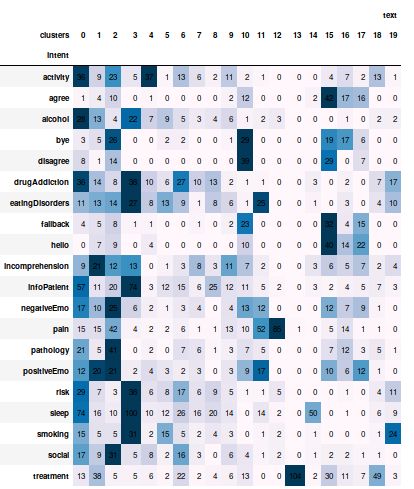
\includegraphics[scale=0.28]{bilstm_ac_cm.png}
	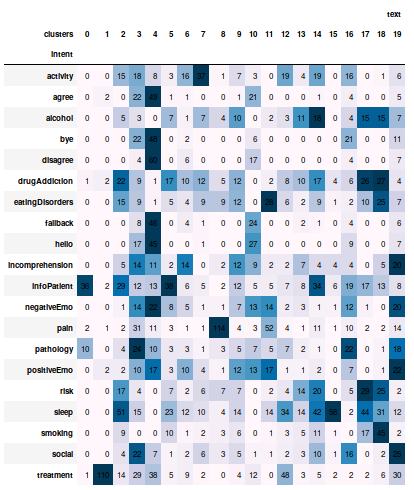
\includegraphics[scale=0.28]{bilstm_gm_cm.png}
	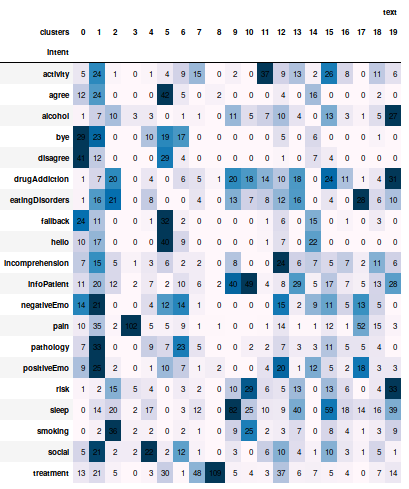
\includegraphics[scale=0.28]{bilstm_km_cm.png}
	\caption{BiLSTM confusion matrixes: : agglomerative clustering, gaussian mixture, Kmeans}
\label{bilstm_gm_cm}
\end{figure}
\FloatBarrier

This model shows really good separatation for {\sc{treatment}} and {\sc{pain}} labels but  
tends to group together utternance belonging to the {\sc{agree, fallback}} and  {\sc{hello}} intent on the one hand and to the  {\sc{bye}} and  {\sc{disagree}} intent on the other.

\subsubsection{Overall comparison}

Table~\ref{final_comparison} summarizes the results, focusing on the best hyper-parameters for each approach and  taking into consideration pretrained GloVe and Google News Word2Vec embeddings. The last two models (LDA and BiLSTM) appear to provide the best results and will therefore be used for further steps.

\begin{table}[htb]
\begin{center}
\begin{tabular}{ |r|c|c|c|c|c| }
\hline
model & features & purity   & silhouette  & homogeneity  & completeness \\ \hline 
Word2Vec 	& 30  & 0.18901 & 0.0695026  & 0.110232  & 0.13267\\ \hline 
GloVe	& 25	& 0.191125  & 0.003554  & 0.110058  & 0.147367 \\ \hline
GloVe 	& 200	& 0.186283  & -0.026413 & 0.102103  & 0.137332 \\ \hline
Google  & 300 	& 0.201614  & -0.016592 & 0.109450  & 0.156423 \\ \hline
LDA 	& 400  	& 0.272718  & 0.192777  & 0.177547  & 0.192270 \\ \hline 
BiLSTM 	& 64  	& \textbf{0.281683}  & 0.22728  & 0.231666  & 0.232176\\ \hline 
\end{tabular}
\end{center}
\caption{Overall comparison}
\label{final_comparison}
\end{table}
\FloatBarrier



\subsection{Classifier}
\label{subsec:classifying2}

In the previous section, we compared different settings for building sentence representations using different methods (LDA, Word2Vec, Glove Embedding etc.) and experimenting with different hyper-parameters. We concluded that the best models were (i) LDA and (ii) biLSTM.

In this section, we now explore how these representations can be used to help guess the corresponding intents and further, how external (forum) data that is automatically labelled using the procedure described in Section~\ref{subsec:dataexpansion} can help improve intent classification.

\subsubsection{Evaluation metrics}

A classical way to evaluate a classification model performance is using accuracy score. Sometimes, especially in case of unbalanced dataset, it can be misleading because it can represent that model learns just one class. It’s better to look for a precision score as a measure of exactness and a recall score as a measure of completeness.

\begin{equation}
P = \frac{TP}{TP+FP} 
\end{equation}

\begin{equation}
R = \frac{TP}{TP+FN}
\end{equation}

where TP - True Positives, FP - False Positives, FN - False Negatives.

If we want to get an idea how our classifier deals with both classes (in simple binary case) we should use F1 score that conveys the balance between the precision and the recall.
\begin{equation}
F1 = \frac{2*P*R}{P+R}
\end{equation}

    There is a cleaner and less ambiguous way to describe the model behaviour that is a confusion matrix. Bigger values on the main diagonal indicate low confusion and good classification accuracy. 

\begin{table}[htb]
\begin{center}
\begin{tabular}{ |r|c|c| }
\hline
& Real positive & Real negative \\ \hline
Predicted positive & True Positive 	& False Positive \\ \hline
Predicted negative & False negative & True negative \\ \hline
\end{tabular}
\caption{Confusion matrix template}
\end{center}
\end{table}
\FloatBarrier

\subsubsection{Training on the Manually Labelled Dataset}

The baseline classifier is trained and tested on the manually labelled
data set using a 60/40 split ratio (65 items for training and 43 for
testing). Both sets are balanced, so that each category is represented
by the same number of items.

We use the SVC classification model and compare two kernels: rbf
(C=10, gamma=1) and linear (C=10, gamma=0.001). For each model, we use
grid search to identify the best parameters and we evaluate using 5
fold cross validation. Table~\ref{tab:classificationresults} shows the results. 

%5-folds Cross Validation error on train set 0.401 + 0.0115 and on test set 0.371 + 0.0338. Small %difference in score indicates good performance and absence of overfitting.

\begin{table}[htb]
\begin{center}
\begin{tabular}{ |p{1.5cm}|p{1cm}|c|c|c|c|c| }
\hline
Model 	& Kernel 	& Train & Test & precision & recall & F1 \\ \hline
\multirow{2}{*}{LDA} &	rbf		& 0.524 + 0.00717 & 0.387 + 0.0341 & 0.308 & 0.316 & 0.287 \\ 
& linear	& 0.371 + 0.00787 & 0.338 + 0.0431 & 0.238 & 0.241 & 0.215 \\ \hline
\multirow{2}{*}{BiLSTM}&	rbf		& 0.418 + 0.0193 & 0.373 + 0.0548 & 0.280 & 0.297 & 0.275 \\ 
& linear	& 0.376 + 0.0147 & 0.343 + 0.0484 & 0.265 & 0.291 & 0.251 \\ \hline
\end{tabular}
\caption{CV score comparison} \label{tab:classificationresults}
\end{center}
\end{table}
\FloatBarrier

\add{What is CV?}

Although the rbf model model has higher scores, the linear one is less prone to overfitting as shown by the small difference between train and test errors. It was decided to try both and observe their behavior.


\subsection{Semi Supervised Learning}
\label{subsec:semisupervised}

We now report on the classifier results produced after each data
expansion step following the procedure described in
Section~\ref{subsec:dataexpansion}.


%Rbf just to next ones: sleep, risk, eatingDisorders, drugAddiction, alcohol, social, activity, smoking, infoPatient, pain, negativeEmo, incomprehension, treatment.

%Linear just to next ones: sleep, risk, eatingDisorders, drugAddiction, social, activity, smoking, alcohol, pain, infoPatient, negativeEmo.
  
\subsubsection{SVC with linear kernel}

For the SVC classifier with linear kernel, we use the following settings.

\begin{itemize}
\item Iteration 0: there is no data expansion. Results show the scores
  obtained for the baseline model (BL) trained on the manually labelled
  data.
\item Iteration 1: Using the we BL model created at iteration 0, we
  label 500 forum sentences for each of the 20 target intents
  yielding a set of 10K labelled sentences. We then cluster these
  sentences into 200 clusters which we then filter using a probability
  threshold of 0.12. After filtering, we have 15 new items per intent.
\item Iteration 2: We repeated the same procedure with a probability
  threshold of 0.1. We obtain 13 new items per intent.
\end{itemize}
%\add{The following sentence is unclear. What do you mean by ``provide expansion to all categories'' ? what shows this ? }: 

As the BiLSTM model did not succeed in providing expansion for all
categories (after labelling all forum sentences, there was no
candidates for some of the intents), we only provide results for the
LDA model. The results are shown in Table~\ref{tab:lin_gen_scores}.

\add{in the tables below: what is ``Score''? If you mean accuracy, you should replace score by accuracy everywhere. Score is vague.}


\begin{table}[htb]
\begin{center}
\begin{tabular}{ |r|c|c|c|c|c|c| }
\hline
Iteration 	& Score  & CV mean & CV std & precision & recall & F1 \\ \hline
0			& 0.2651 & 0.337   & 0.0503 & 0.265 	& 0.340  & 0.262 \\ \hline
1			& 0.2895 & 0.323   & 0.0212 & 0.289 	& 0.319  & 0.290 \\ \hline
2 			& 0.3174 & 0.333   & 0.0118 & 0.317 	& 0.325  & 0.304 \\ \hline
\end{tabular}
\caption{Classifier scores comparison}
\label{tab:lin_gen_scores}
\end{center}
\end{table}
\FloatBarrier

\begin{table}[htb]
\begin{center}
\begin{tabular}{ |r|c|c|c|l|c|c|c|l|c|c|c| }
\hline
label 			& \multicolumn{3}{c|}{precision} && \multicolumn{3}{c|}{recall} && \multicolumn{3}{c|}{f1} \\ \hline 
activity 		&  0.56 & 0.30 & 0.42 && 0.36 & 0.27 & 0.29 && 0.44 & 0.28 & 0.34 \\ \hline 
agree 			&  0.23 & 0.16 & 0.05 && 0.19 & 0.28 & 0.12 && 0.21 & 0.21 & 0.07 \\ \hline 
alcohol 		&  0.35 & 0.53 & 0.56 && 0.34 & 0.44 & 0.49 && 0.34 & 0.48 & 0.52 \\ \hline 
bye 			&  0.14 & 0.33 & 0.53 && 0.24 & 0.41 & 0.38 && 0.18 & 0.36 & 0.44 \\ \hline 
disagree 		&  0.14 & 0.14 & 0.37 && 0.40 & 0.08 & 0.38 && 0.21 & 0.10 & 0.38 \\ \hline 
drugAddiction 	&  0.21 & 0.21 & 0.23 && 0.12 & 0.29 & 0.23 && 0.15 & 0.24 & 0.23 \\ \hline 
eatingDisorders &  0.26 & 0.37 & 0.28 && 0.61 & 0.73 & 0.34 && 0.36 & 0.49 & 0.31 \\ \hline 
fallback 		&  0.05 & 0.12 & 0.00 && 0.09 & 0.31 & 0.00 && 0.06 & 0.17 & 0.00 \\ \hline 
hello 			&  0.05 & 0.00 & 0.21 && 0.17 & 0.00 & 0.43 && 0.07 & 0.00 & 0.28 \\ \hline 
incomprehension &  0.49 & 0.37 & 0.35 && 0.20 & 0.26 & 0.20 && 0.29 & 0.31 & 0.25 \\ \hline 
infoPatient 	&  0.33 & 0.49 & 0.49 && 0.25 & 0.34 & 0.44 && 0.29 & 0.40 & 0.46 \\ \hline 
negativeEmo 	&  0.12 & 0.05 & 0.16 && 0.21 & 0.06 & 0.21 && 0.15 & 0.05 & 0.18 \\ \hline 
pain 			&  0.70 & 0.60 & 0.70 && 0.81 & 0.46 & 0.81 && 0.75 & 0.53 & 0.75 \\ \hline 
pathology 		&  0.02 & 0.05 & 0.05 && 0.50 & 0.09 & 0.29 && 0.04 & 0.06 & 0.08 \\ \hline 
positiveEmo 	&  0.28 & 0.37 & 0.09 && 0.07 & 0.11 & 0.14 && 0.11 & 0.17 & 0.11 \\ \hline 
risk 			&  0.02 & 0.12 & 0.07 && 0.08 & 0.16 & 0.11 && 0.04 & 0.13 & 0.08 \\ \hline 
sleep 			&  0.44 & 0.42 & 0.49 && 0.47 & 0.50 & 0.54 && 0.46 & 0.46 & 0.51 \\ \hline 
smoking 		&  0.60 & 0.44 & 0.49 && 0.68 & 0.59 & 0.66 && 0.64 & 0.51 & 0.56 \\ \hline 
social 			&  0.14 & 0.14 & 0.26 && 0.20 & 0.21 & 0.31 && 0.16 & 0.17 & 0.28 \\ \hline 
treatment		&  0.19 & 0.58 & 0.56 && 0.80 & 0.75 & 0.15 && 0.30 & 0.67 & 0.24 \\ \hline 
\end{tabular}
\caption{Comparison of classification scores for SVC with linear kernel}
\label{tab:results-svc-linear}
\end{center}
\end{table}
\FloatBarrier

As can be seen from Table \ref{tab:lin_gen_scores}, scores on the gold
test dataset, precision and F1 score are steadily increasing (although
values for CV score and recall are not stable\add{what does this mean?
  what is CV?}.  From Figure \ref{lsvc_cm}, we can also see that the
confusion matrix became more diagonalized although categories that
were confusing from the very begining ({\sc{agree, diasagree, fallback,
hello, negativeEmo, positiveEmo, risk, alcohol}}) are still mixed
together. Coming back to section \ref{subsec:lda}, we can see that
these categories were considered to be in the same cluster, so on that
early stage it was possible to predict such outcome. On the other hand
the predictions for such intents as {\sc{social, incomprehension, infoPatient, treatment}} improves.

\begin{figure}[h]
	\centering
	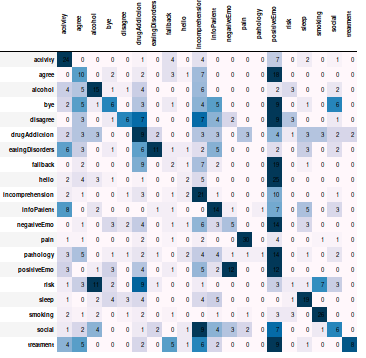
\includegraphics[scale=0.3]{lsvc_0.png}
	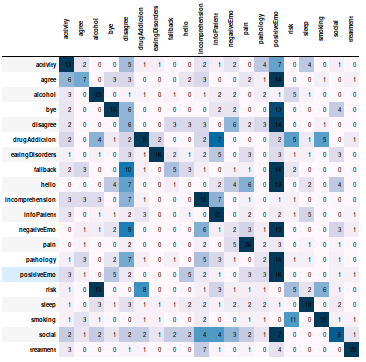
\includegraphics[scale=0.3]{lsvc_1.png}
	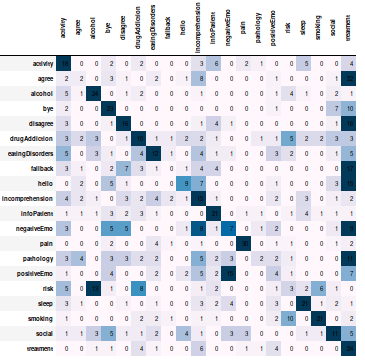
\includegraphics[scale=0.3]{lsvc_2.png}
	\caption{SVC confusion matrix for iteration 0, 1, 2.}
\label{lsvc_cm}
\end{figure}
\FloatBarrier




\subsubsection{SVC with rbf kernel}
\label{subsec:semisupervised-rbf}


\begin{itemize}
\item Iteration 0: there is no data expansion. Results show the scores
  obtained for the baseline model (BL) trained on the manually labelled
  data.
\item Iteration 1: Using the we BL model created at iteration 0, we
  label 500 forum sentences for each of the 20 target intents
  yielding a set of 10K labelled sentences. We then cluster these
  sentences into 1000 clusters which we then filter using a probability
  threshold of 0.15. After filtering, we have 6 new items per intent.
\item Iteration 2: We repeated the same procedure with a probability
  threshold of 0.11. We obtain 5 new items per intent.
\end{itemize}

\begin{table}[htb]
\begin{center}
\begin{tabular}{ |r|c|c|c|c|c|c| }
\hline
Iteration 	& Score  & CV mean & CV std & precision & recall & F1 \\ \hline
0			& 0.3186 & 0.371   & 0.0338 & 0.308 	& 0.316  & 0.287 \\ \hline
1			& 0.3523 & 0.350   & 0.0153 & 0.352 	& 0.371  & 0.346 \\ \hline
2 			& 0.3167 & 0.332   & 0.0150 & 0.316 	& 0.331  & 0.313 \\ \hline
\end{tabular}
\caption{Classifier scores comparison}
\label{tab:rbf_gen_scores}
\end{center}
\end{table}
\FloatBarrier

\begin{table}[htb]
\centering
\begin{tabular}{ |r|c|c|c|l|c|c|c|l|c|c|c| }
\hline
label 			& \multicolumn{3}{c|}{precision} && \multicolumn{3}{c|}{recall} && \multicolumn{3}{c|}{f1} \\ \hline 
				& it 0 &  it 1 & it 2 && it 0 & it 1 & it 2 && it 0 & it 1 & it 2\\ \hline 
activity 		& 0.44 &  0.49 & 0.37 && 0.40 & 0.54 & 0.34 && 0.42 & 0.51 & 0.36\\ \hline 
agree 			& 0.72 &  0.23 & 0.14 && 0.20 & 0.31 & 0.21 && 0.32 & 0.27 & 0.17\\ \hline 
alcohol 		& 0.51 &  0.56 & 0.47 && 0.44 & 0.41 & 0.39 && 0.47 & 0.47 & 0.43\\ \hline 
bye 			& 0.35 &  0.56 & 0.33 && 0.29 & 0.67 & 0.30 && 0.32 & 0.39 & 0.31\\ \hline 
disagree 		& 0.33 &  0.33 & 0.35 && 0.38 & 0.31 & 0.43 && 0.35 & 0.32 & 0.38\\ \hline 
drugAddiction 	& 0.09 &  0.26 & 0.28 && 0.13 & 0.39 & 0.29 && 0.11 & 0.31 & 0.28\\ \hline 
eatingDisorders & 0.33 &  0.47 & 0.33 && 0.45 & 0.67 & 0.25 && 0.38 & 0.52 & 0.28\\ \hline 
fallback 		& 0.00 &  0.26 & 0.14 && 0.00 & 0.12 & 0.12 && 0.00 & 0.17 & 0.13\\ \hline 
hello 			& 0.23 &  0.51 & 0.40 && 0.25 & 0.25 & 0.19 && 0.24 & 0.34 & 0.26\\ \hline 
incomprehension & 0.51 &  0.30 & 0.42 && 0.29 & 0.29 & 0.43 && 0.37 & 0.30 & 0.42\\ \hline 
infoPatient 	& 0.30 &  0.42 & 0.37 && 0.54 & 0.35 & 0.52 && 0.39 & 0.38 & 0.43\\ \hline 
negativeEmo 	& 0.12 &  0.05 & 0.14 && 0.19 & 0.06 & 0.18 && 0.14 & 0.05 & 0.16\\ \hline 
pain 			& 0.30 &  0.65 & 0.49 && 0.22 & 0.49 & 0.44 && 0.25 & 0.56 & 0.46\\ \hline 
pathology 		& 0.09 &  0.14 & 0.16 && 0.16 & 0.35 & 0.29 && 0.12 & 0.20 & 0.21\\ \hline 
positiveEmo 	& 0.09 &  0.14 & 0.16 && 0.17 & 0.20 & 0.20 && 0.12 & 0.16 & 0.18\\ \hline 
risk 			& 0.05 &  0.07 & 0.05 && 0.17 & 0.14 & 0.11 && 0.07 & 0.09 & 0.06\\ \hline 
sleep 			& 0.42 &  0.58 & 0.56 && 0.58 & 0.66 & 0.63 && 0.49 & 0.62 & 0.59\\ \hline 
smoking 		& 0.65 &  0.51 & 0.58 && 0.61 & 0.54 & 0.54 && 0.63 & 0.52 & 0.56\\ \hline 
social 			& 0.33 &  0.19 & 0.21 && 0.50 & 0.29 & 0.56 && 0.49 & 0.23 & 0.31\\ \hline 
treatment 		& 0.51 &  0.63 & 0.40 && 0.35 & 0.40 & 0.22 && 0.42 & 0.49 & 0.28\\ \hline 
\end{tabular}
\caption{Comparison of classification scores for SVC with rbf kernel}
\end{table}
\FloatBarrier

Although scores (Table \ref{tab:rbf_gen_scores}) decrease on the second iteration, the confusion matrix becomes more diagonalized (Figure \ref{rbf_svc_cm}) and F1 increases. Intents as{\sc{drugAddiction, disagree}} are better classified just after the first iteration. Some confusing groups like {\sc{agree, bye, diasgree, fallback, hello}} and {\sc{positiveEmo, negativeEmo}} or {\sc{risk, alcohol}} still tends to stay together.

\begin{figure}[h]
	\centering
	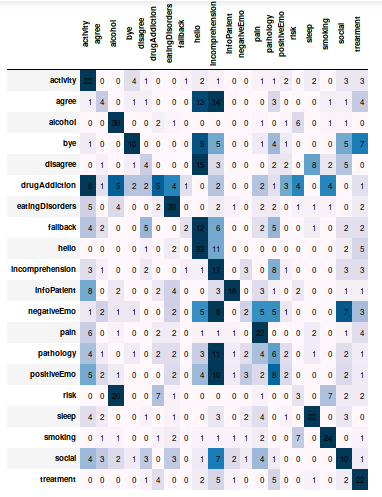
\includegraphics[scale=0.25]{svc0_cm.png}
	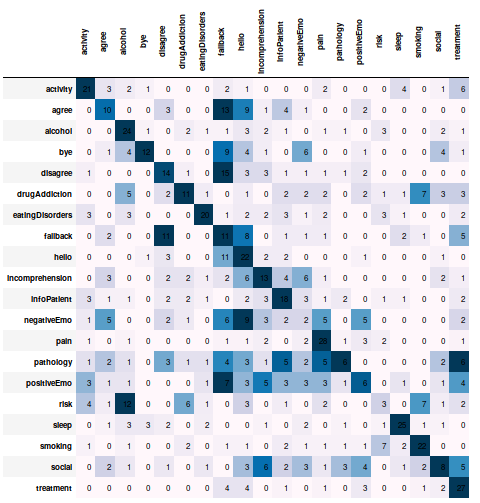
\includegraphics[scale=0.25]{svc1_cm.png}
	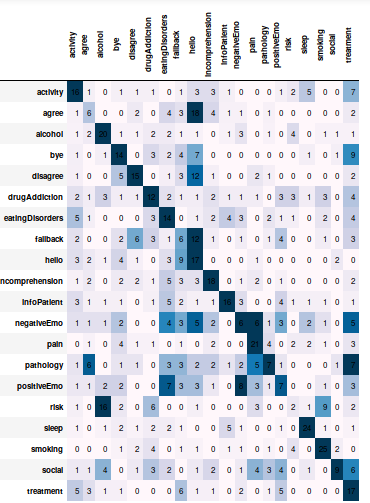
\includegraphics[scale=0.25]{svc2_cm.png}
	\caption{SVC confusion matrix for iteration 0, 1, 2.}
\label{rbf_svc_cm}
\end{figure}
\FloatBarrier


\section{Conclusion and future work}
\label{sec:conclusion}

In this project, we were dealing with task of semi-supervised text
classification for expanding initial dataset. Our approach is to train
a sentence representation model that will be able to provide clusters
similar to initial classes. For this purpose we used LDA, W2V and
BiLSTM models and evaluated them with the help of clustering
scores. We then trained SVC and Kmeans models to label external,
forum, data and chose the best examples to extend existing
dataset and update models with them.

%% In this project we were dealing with task of paraphrase detection for expanding initial dataset. Our approch is to train the word embedding model that will be able to provide clusters similar to initial classes. We used LDA and Word2Vec models for that and later trained SVC and Kmeans models to label external data and chose the representative example to extend existing dataset and retrain models on it.

Our results show how algorithm tends to converge and to be more
precise though high rate of confusion between labels in intial
classifier increases this confusion in futher data expansion. This
confusion can be measured before going through semi-supervised routine
in order to achive acceptable level or eliminate some intents. Also,
the more data you have the higher chances to find more similar
sentences to initial one so that possible context for each intent will
grow gradually while diversified data can cause even more perplexity.

Future work will be devoted to (i) improving the sentence
representation models using neural methods such as for instance the
recent BERT word embeddings \cite{devlin2018bert}; and (ii) investigating one-shot \cite{koch2015siamese} and transfer learning approaches \cite{huang2017zero} to improve classification
scores.

To handle real life examples, further directions include the development of classifiers which (i) label a user utterance with both an intent and a set of attribute-value pairs as illustrated in Figure~\ref{fig:rasa}; and (ii) can handle utterances with multiple intents. 

%% Another direction is the development of a classifier As user utterances in fact often denote not a single but multiple intents,  Transfering from
%% one-intent to multi-intent is preferable due to the fact that
%% sentences are usually ambiguous than not. Another possible direction
%% is developing a framework for adding new labels to the existing
%% classifier.

\bibliographystyle{alpha}

\bibliography{biblio}

\clearpage
\section{Supplemental materials}

\subsection{Iterations with SVC with linear kernel}
\begin{table}[htb]
\begin{center}
\begin{tabular}{ |r|c|c|c|c|c|c| }
\hline
label 			& precision & recall & f1-score & support\\ \hline 
\\ \hline 
activity 		&  0.56 & 0.36 & 0.44 &   66\\ \hline 
agree 			&  0.23 & 0.19 & 0.21 &   54\\ \hline 
alcohol 		&  0.35 & 0.34 & 0.34 &   44\\ \hline 
bye 			&  0.14 & 0.24 & 0.18 &   25\\ \hline 
disagree 		&  0.14 & 0.40 & 0.21 &   15\\ \hline 
drugAddiction 	&  0.21 & 0.12 & 0.15 &   75\\ \hline 
eatingDisorders &  0.26 & 0.61 & 0.36 &   18\\ \hline 
fallback 		&  0.05 & 0.09 & 0.06 &   22\\ \hline 
hello 			&  0.05 & 0.17 & 0.07 &   12\\ \hline 
incomprehension &  0.49 & 0.20 & 0.29 &  103\\ \hline 
infoPatient 	&  0.33 & 0.25 & 0.29 &   55\\ \hline 
negativeEmo 	&  0.12 & 0.21 & 0.15 &   24\\ \hline 
pain 			&  0.70 & 0.81 & 0.75 &   37\\ \hline 
pathology 		&  0.02 & 0.50 & 0.04 &    2\\ \hline 
positiveEmo 	&  0.28 & 0.07 & 0.11 &  178\\ \hline 
risk 			&  0.02 & 0.08 & 0.04 &   12\\ \hline 
sleep 			&  0.44 & 0.47 & 0.46 &   40\\ \hline 
smoking 		&  0.60 & 0.68 & 0.64 &   38\\ \hline 
social 			&  0.14 & 0.20 & 0.16 &   30\\ \hline 
treatment		&  0.19 & 0.80 & 0.30 &   10\\ \hline 
\\ \hline 
micro avg 		&  0.27 & 0.27 & 0.27 &  860\\ \hline 
macro avg 		&  0.27 & 0.34 & 0.26 &  860\\ \hline 
weighted avg 	&  0.33 & 0.27 & 0.27 &  860\\ \hline 
\end{tabular}
\caption{Classifier 0}
\end{center}
\end{table}
\FloatBarrier

\begin{figure}[h]
	\centering
	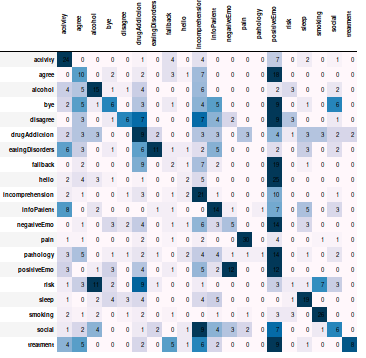
\includegraphics[scale=0.7]{lsvc_0.png}
	\caption{SVC confusion matrix for iteration 0.}
\label{lsvc_cm_0}
\end{figure}
\FloatBarrier



\begin{table}[htb]
\begin{center}
\begin{tabular}{ |r|c|c|c|c|c|c| }
label 			& precision & recall & f1-score & support\\ \hline 
\\ \hline 
activity 		&  0.30 & 0.27 & 0.28 &   49\\ \hline 
agree 			&  0.16 & 0.28 & 0.21 &   25\\ \hline 
alcohol 		&  0.53 & 0.44 & 0.48 &   52\\ \hline 
bye 			&  0.33 & 0.41 & 0.36 &   34\\ \hline 
disagree 		&  0.14 & 0.08 & 0.10 &   78\\ \hline 
drugAddiction 	&  0.21 & 0.29 & 0.24 &   31\\ \hline 
eatingDisorders &  0.37 & 0.73 & 0.49 &   22\\ \hline 
fallback 		&  0.12 & 0.31 & 0.17 &   16\\ \hline 
hello 			&  0.00 & 0.00 & 0.00 &   19\\ \hline 
incomprehension &  0.37 & 0.26 & 0.31 &   61\\ \hline 
infoPatient 	&  0.49 & 0.34 & 0.40 &   61\\ \hline 
negativeEmo 	&  0.05 & 0.06 & 0.05 &   31\\ \hline 
pain 			&  0.60 & 0.46 & 0.53 &   56\\ \hline 
pathology 		&  0.05 & 0.09 & 0.06 &   23\\ \hline 
positiveEmo 	&  0.37 & 0.11 & 0.17 &  142\\ \hline 
risk 			&  0.12 & 0.16 & 0.13 &   32\\ \hline 
sleep 			&  0.42 & 0.50 & 0.46 &   36\\ \hline 
smoking 		&  0.44 & 0.59 & 0.51 &   32\\ \hline 
social 			&  0.14 & 0.21 & 0.17 &   28\\ \hline 
treatment 		&  0.58 & 0.78 & 0.67 &   32\\ \hline 
\\ \hline 
micro avg 		&  0.29 & 0.29 & 0.29 &  860\\ \hline 
macro avg 		&  0.29 & 0.32 & 0.29 &  860\\ \hline 
weighted avg 	&  0.33 & 0.29 & 0.29 &  860\\ \hline
\end{tabular}
\caption{Classifier 1}
\end{center}
\end{table}
\FloatBarrier

\begin{figure}[h]
	\centering
	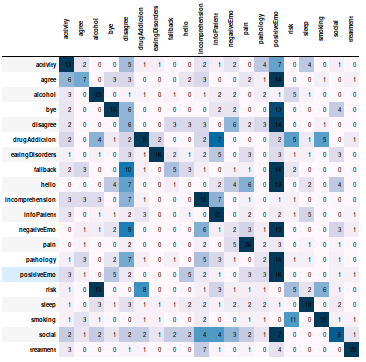
\includegraphics[scale=0.7]{lsvc_1.png}
	\caption{SVC confusion matrix for iteration 1.}
\label{lsvc_cm_1}
\end{figure}
\FloatBarrier



\begin{table}[htb]
\begin{center}
\begin{tabular}{ |r|c|c|c|c|c|c| }
label  			&    precision  &  recall & f1-score &  support\\ \hline 
\\ \hline 
activity 		&  0.42 & 0.29 & 0.34 &   63\\ \hline 
agree 			&  0.05 & 0.12 & 0.07 &   17\\ \hline 
alcohol 		&  0.56 & 0.49 & 0.52 &   49\\ \hline 
bye 			&  0.53 & 0.38 & 0.44 &   61\\ \hline 
disagree 		&  0.37 & 0.38 & 0.38 &   42\\ \hline 
drugAddiction 	&  0.23 & 0.23 & 0.23 &   43\\ \hline 
eatingDisorders &  0.28 & 0.34 & 0.31 &   35\\ \hline 
fallback 		&  0.00 & 0.00 & 0.00 &    6\\ \hline 
hello 			&  0.21 & 0.43 & 0.28 &   21\\ \hline 
incomprehension &  0.35 & 0.20 & 0.25 &   76\\ \hline 
infoPatient 	&  0.49 & 0.44 & 0.46 &   48\\ \hline 
negativeEmo 	&  0.16 & 0.21 & 0.18 &   34\\ \hline 
pain 			&  0.70 & 0.81 & 0.75 &   37\\ \hline 
pathology 		&  0.05 & 0.29 & 0.08 &    7\\ \hline 
positiveEmo 	&  0.09 & 0.14 & 0.11 &   29\\ \hline 
risk 			&  0.07 & 0.11 & 0.08 &   28\\ \hline 
sleep 			&  0.49 & 0.54 & 0.51 &   39\\ \hline 
smoking 		&  0.49 & 0.66 & 0.56 &   32\\ \hline 
social 			&  0.26 & 0.31 & 0.28 &   36\\ \hline 
treatment 		&  0.56 & 0.15 & 0.24 &  157\\ \hline 
\\ \hline 
micro avg 		&  0.32 & 0.32 & 0.32 &  860\\ \hline 
macro avg 		&  0.32 & 0.32 & 0.30 &  860\\ \hline 
weighted avg 	&  0.40 & 0.32 & 0.33 &  860\\ \hline 
\end{tabular}
\caption{Classifier 2}
\end{center}
\end{table}
\FloatBarrier

\begin{figure}[h]
	\centering
	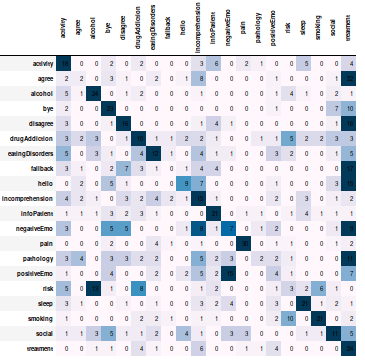
\includegraphics[scale=0.7]{lsvc_2.png}
	\caption{SVC confusion matrix for iteration 2.}
\label{lsvc_cm_2}
\end{figure}
\FloatBarrier



\subsection{Iterations with SVC with rbf kernel}

\begin{table}[htb]
\begin{center}
\begin{tabular}{ |r|c|c|c|c| }
\hline
label 			& precision & recall & f1-score & support\\ \hline 
activity 		& 0.44 & 0.40 & 0.42 &  47\\ \hline 
agree 			& 0.72 & 0.20 & 0.32 & 152\\ \hline 
alcohol 		& 0.51 & 0.44 & 0.47 &  50\\ \hline 
bye 			& 0.35 & 0.29 & 0.32 &  51\\ \hline 
disagree 		& 0.33 & 0.38 & 0.35 &  37\\ \hline 
drugAddiction 	& 0.09 & 0.13 & 0.11 &  30\\ \hline 
eatingDisorders & 0.33 & 0.45 & 0.38 &  31\\ \hline 
fallback 		& 0.00 & 0.00 & 0.00 &   8\\ \hline 
hello 			& 0.23 & 0.25 & 0.24 &  40\\ \hline 
incomprehension & 0.51 & 0.29 & 0.37 &  76\\ \hline 
infoPatient 	& 0.30 & 0.54 & 0.39 &  24\\ \hline 
negativeEmo 	& 0.12 & 0.19 & 0.14 &  26\\ \hline 
pain 			& 0.30 & 0.22 & 0.25 &  59\\ \hline 
pathology 		& 0.09 & 0.16 & 0.12 &  25\\ \hline 
positiveEmo 	& 0.09 & 0.17 & 0.12 &  24\\ \hline 
risk 			& 0.05 & 0.17 & 0.07 &  12\\ \hline 
sleep 			& 0.42 & 0.58 & 0.49 &  31\\ \hline 
smoking 		& 0.65 & 0.61 & 0.63 &  46\\ \hline 
social 			& 0.33 & 0.50 & 0.39 &  28\\ \hline 
treatment 		& 0.51 & 0.35 & 0.42 &  63\\ \hline 
\\ \hline 
micro avg 		& 0.32 & 0.32 & 0.32 & 860\\ \hline 
macro avg 		& 0.32 & 0.32 & 0.30 & 860\\ \hline 
weighted avg 	& 0.42 & 0.32 & 0.34 & 860\\ \hline 
\end{tabular}
\caption{Classification report for 0 iteration}
\end{center}
\end{table}
\FloatBarrier

\begin{figure}[h]
	\centering
	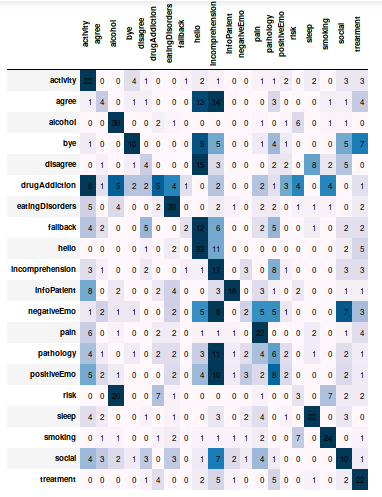
\includegraphics[scale=0.7]{svc0_cm.png}
	\caption{SVC confusion matrix for iteration 0.}
\label{svc_cm_0}
\end{figure}
\FloatBarrier


\begin{table}[htb]
\begin{center}
\begin{tabular}{ |r|c|c|c|c| }
\hline
label 			& precision & recall & f1-score &  support\\ \hline 
\\ \hline 
activity 		&  0.49 & 0.54 & 0.51 &   39\\ \hline 
agree 			&  0.23 & 0.31 & 0.27 &   32\\ \hline 
alcohol 		&  0.56 & 0.41 & 0.47 &   59\\ \hline 
bye 			&  0.28 & 0.67 & 0.39 &   18\\ \hline 
disagree 		&  0.33 & 0.31 & 0.32 &   45\\ \hline 
drugAddiction 	&  0.26 & 0.39 & 0.31 &   28\\ \hline 
eatingDisorders &  0.47 & 0.67 & 0.55 &   30\\ \hline 
fallback 		&  0.26 & 0.12 & 0.17 &   88\\ \hline 
hello 			&  0.51 & 0.25 & 0.34 &   88\\ \hline 
incomprehension &  0.30 & 0.29 & 0.30 &   45\\ \hline 
infoPatient 	&  0.42 & 0.35 & 0.38 &   52\\ \hline 
negativeEmo 	&  0.05 & 0.06 & 0.05 &   36\\ \hline 
pain 			&  0.65 & 0.49 & 0.56 &   57\\ \hline 
pathology 		&  0.14 & 0.35 & 0.20 &   17\\ \hline 
positiveEmo 	&  0.14 & 0.20 & 0.16 &   30\\ \hline 
risk 			&  0.07 & 0.14 & 0.09 &   21\\ \hline 
sleep 			&  0.58 & 0.66 & 0.62 &   38\\ \hline 
smoking 		&  0.51 & 0.54 & 0.52 &   41\\ \hline 
social 			&  0.19 & 0.29 & 0.23 &   28\\ \hline 
treatment 		&  0.63 & 0.40 & 0.49 &   68\\ \hline 
\\ \hline 
micro avg 		&  0.35 & 0.35 & 0.35 &  860\\ \hline 
macro avg 		&  0.35 & 0.37 & 0.35 &  860\\ \hline 
weighted avg 	&  0.40 & 0.35 & 0.36 &  860\\ \hline 
\end{tabular}
\caption{Classification report for the first iteration}
\end{center}
\end{table}
\FloatBarrier

\begin{figure}[h]
	\centering
	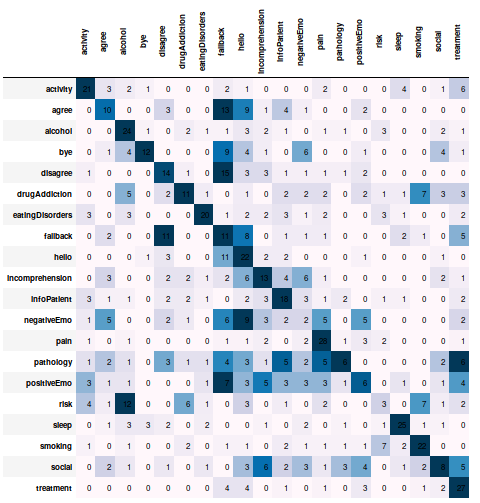
\includegraphics[scale=0.7]{svc1_cm.png}
	\caption{SVC confusion matrix for iteration 1.}
\label{svc_cm_1}
\end{figure}
\FloatBarrier


\begin{table}[htb]
\begin{center}
\begin{tabular}{ |r|c|c|c|c| }
\hline
label  &    precision & recall & f1-score  & support\\ \hline 
\\ \hline 
activity 		& 0.37 &   0.34 &   0.36 & 47\\ \hline 
agree 			& 0.14 &   0.21 &   0.17 & 29\\ \hline 
alcohol 		& 0.47 &   0.39 &   0.43 & 51\\ \hline 
bye 			& 0.33 &   0.30 &   0.31 & 46\\ \hline 
disagree 		& 0.35 &   0.43 &   0.38 & 35\\ \hline 
drugAddiction 	& 0.28 &   0.29 &   0.28 & 42\\ \hline 
eatingDisorders & 0.33 &   0.25 &   0.28 & 57\\ \hline 
fallback 		& 0.14 &   0.12 &   0.13 & 51\\ \hline 
hello 			& 0.40 &   0.19 &   0.26 & 90\\ \hline 
incomprehension & 0.42 &   0.43 &   0.42 & 42\\ \hline 
infoPatient 	& 0.37 &   0.52 &   0.43 & 31\\ \hline 
negativeEmo 	& 0.14 &   0.18 &   0.16 & 34\\ \hline 
pain 			& 0.49 &   0.44 &   0.46 & 48\\ \hline 
pathology 		& 0.16 &   0.29 &   0.21 & 24\\ \hline 
positiveEmo 	& 0.16 &   0.20 &   0.18 & 35\\ \hline 
risk 			& 0.05 &   0.11 &   0.06 & 19\\ \hline 
sleep 			& 0.56 &   0.63 &   0.59 & 38\\ \hline 
smoking 		& 0.58 &   0.54 &   0.56 & 46\\ \hline 
social 			& 0.21 &   0.56 &   0.31 & 16\\ \hline 
treatment 		& 0.40 &   0.22 &   0.28 & 79\\ \hline 
\\ \hline 
micro avg &    0.32 &   0.32 &   0.32 &    860\\ \hline 
macro avg &    0.32 &   0.33 &   0.31 &    860\\ \hline 
weighted avg & 0.34 &   0.32 &   0.32 &    860\\ \hline 
\\ \hline 
\end{tabular}
\caption{Classification report for the second iteration}
\end{center}
\end{table}
\FloatBarrier

\begin{figure}[h]
	\centering
	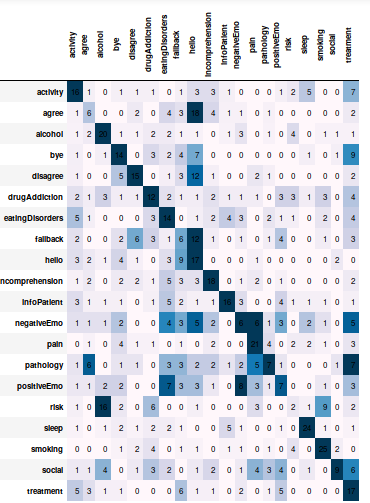
\includegraphics[scale=0.7]{svc2_cm.png}
	\caption{SVC confusion matrix for iteration 2.}
\label{svc_cm_2}
\end{figure}
\FloatBarrier

\end{document}
